\documentclass[10pt,a4paper]{article}
\usepackage[a4paper, total={7in, 8in}]{geometry}

\usepackage[utf8]{inputenc}
\usepackage[T1]{fontenc}
\usepackage[export]{adjustbox}
\usepackage[french]{babel}
\usepackage{graphicx}
\usepackage{eso-pic}
\usepackage{transparent}
\usepackage[export]{adjustbox}

\usepackage[nonumberlist]{glossaries}
\usepackage{glossaries}
\usepackage{imakeidx}

% 1 : Logo ulb en fond
\newcommand\BackgroundPic{%
    \put(0,-47){%
        \parbox[b][\paperheight]{\paperwidth}{%
            \vfill
            \centering
            {\transparent{0.09}
\includegraphics[width=1.17 \textwidth]{Fondulb.jpg}}%
            \vfill
        }
    }
}





% Glossaire
\newglossaryentry{Tower Defense}
{
	name=Tower Defense,
    description={Jeu de stratégie où le but est de défendre la zone d'un \gls{joueur} contre des vagues  successives d'ennemis\index{ennemis} en construisant et en améliorant progressivement ses tours.}
}
\newglossaryentry{joueur}
{
	name=joueur,
    description={Personnage fictif du jeux qu'incarne l'\gls{utilisateur}}
}

\newglossaryentry{utilisateur}
{
	name=utilisateur,
    description={Personnage réel qui joue à Meatwars: Revenge of the Falling Vegan}
}

\newglossaryentry{compte}
{
	name=compte,
    description={Contient toutes les données de l'\gls{utilisateur}}
}

\newglossaryentry{serveur}
{
	name=serveur,
    description={Programme qui réceptionne les connections des \glspl{client}. Il a les données de tous les \glspl{utilisateur}}
}

\newglossaryentry{client}
{
	name=client,
    description={Programme que l'\gls{utilisateur} lance pour se connecter au \gls{serveur}. Il permet à l'\gls{utilisateur} de jouer au jeu via le terminal ou l'interface graphique}
}
\makeglossaries
\setglossarysection{subsection}


\makeindex
\indexsetup{level=\chapter}
% Pour ajouter un mot à l'index: "\index{mot}"



\begin{document}
\AddToShipoutPicture*{\BackgroundPic}

\begin{titlepage}
\begin{center}
\vspace*{-1.5cm}

\includegraphics[width=8cm]{ulb.pdf}
\vspace{6cm}

\par{\huge \textbf{SRD: Tower Defense}}\bigbreak
\bigbreak
\par{\huge \textbf{\textit{{Meat war: Rise of the fallen vegan}}}}
\vspace{2cm}
\par{\large [Cours: INFO-F-209]}
\vspace{2cm}

\par \hrulefill \par
\vspace{1cm}
\bsc{Jacobs} Alexandre 
\bsc{\&}
\bsc{Innocent} Antoine
\bsc{\&}
\bsc{André} Bob
\bsc{\&}
\bsc{Vangeem} Nicolas
\bsc{\&}
\bsc{Roos} Kim
\bsc{\&}
\bsc{Paquet} Michael
\bsc{\&}
\bsc{Singh} Sundeep
{\emph \\BA2 Informatique}
\vspace{0.7cm}
\par \hrulefill \par

\vspace{2cm}
\par Décembre 2016

\end{center}
\end{titlepage}
\newpage
\tableofcontents
\newpage

\section{Introduction}
\subsection{But du projet}

\noindent Ce document joue le role du document de spécification des besoins ou SRD (System requirement Document) pour le projet INFO-F209 : "Meat war: Rise of the falling vegan".
	Ces exigences portent sur un travail de groupe (8 personnes) codé majoritairement en C++ avec une section C pour le \gls{serveur}. Le produit final est donc un jeu de type Tower Defense multijoueur en réseau.
Ce jeu n'ayant aucun but lucratif, nous considerons le \gls{client} principal comme étant le \gls{joueur} du jeux en question.
Ainsi, ce document présente des spécifications propres à l'\gls{utilisateur} et propre au système. Celui-ci va également mettre en avant la communication \gls{client}/\gls{serveur} afin de bien mettre en place l'aspect multijoueur réseau du produit. 

\subsection{Cadre}

\noindent Ce document ne varie pas en fonction des differentes architectures ou systèmes d'exploitation.

% Glossaire
\glsaddall
\printglossary[numberedsection]

\subsection{Historique de document}

\begin{center}
\hspace*{0cm}
\begin{tabular}{|c|c|c|c|}
\hline
Versions & Auteur & Date & Modifications \\
\hline
0.0 & Alexandre \& Antoine & 10-12-2016 & Création de la structure du document\\
0.1 & Sundeep \& Michael & 10-12-2016 & Ajout des use cases et diagrammes d'activité au niveau utilisateur.\\
0.2 & Équipe & 16-12-2016 & Ajout des besoins d'utilisateur et besoins du système\\
0.3 & Kim & 16-12-2016 & Ajout du glossaire et de l'index\\
1.0 & Équipe & 19-12-2016 & \textbf{Deadline pour la phase 1}\\
\hline
\end{tabular}
\end{center}

% version plus simple de l'historique du document
%\begin{description}
%	\item[0.1] [10-12-2016] - Création de la structure du document - Alexandre \& Antoine
%    \item[0.2] [10-12-2016] - Ajout des use cases et diagrammes d'activité au niveau utilisateur - Sundeep \& Mickael
%    \item[0.3] [16-12-2016] - Ajout du glossaire et de l'index - Kim
%    \item[1.0] [19-12-2016] - \textbf{Deadline pour la phase 1 - Équipe}
%\end{description}

\newpage
\section{Besoins de l'utilisateur}

\noindent Les besoins de l'\gls{utilisateur} seront expliqués au travers de plusieurs graphes/explications, en voici ici un résumé.\\
Le but de l'application est de permettre à l'\gls{utilisateur} de pouvoir jouer à un jeu de type Tower Defense. Celui-ci sera disponible depuis un menu\index{menu} accessible après connexion et offrira au \gls{client} plusieurs services. En effet, l'\gls{utilisateur} devra se créer un \gls{compte} avant d'avoir accès au menu.\\
Il pourra alors consulter son profil\index{consulter son profil} ainsi que celui de ses amis, et modifier le sien à souhait (pseudo, avatar, ...).
Un classement\index{classement} sera également accessible et permettra de situer un \gls{joueur} par rapport à un autre en fonction de leur score respectif.\\
Comme dit implicitement plus haut, l'\gls{utilisateur} disposera d'une liste d'amis\index{liste d'amis} avec qui il lui sera possible de discuter via une fenêtre de conversation.\\

\noindent Le menu\index{menu} permettra bien évidemment enfin de créer une partie\index{partie} afin de jouer au jeu. Niveau de difficulté, mode, et nombre de \glspl{joueur} (au maximum de 4) seront spécifiés par le \gls{client} avant que celui-ci ne lance la partie\index{partie}. Une seule et unique carte sera cependant disponible.
\subsection{Exigences fonctionnelles}
\subsubsection{Use case: menu\index{menu}}
\begin{center}
    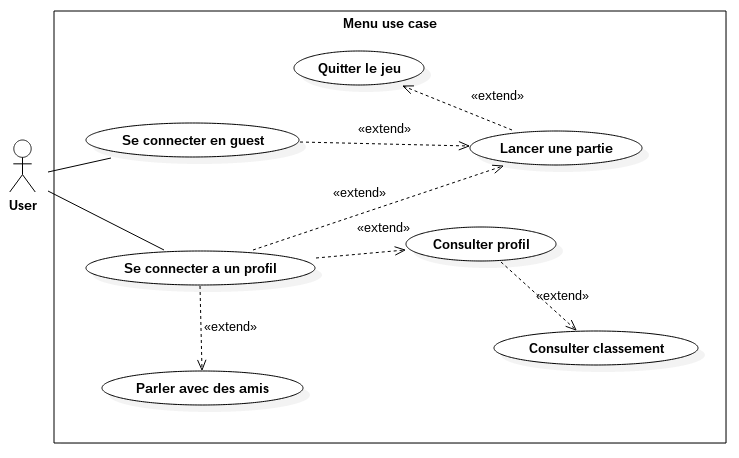
\includegraphics[height=12cm,width=16.45cm]{menu_use_case.png}
\end{center}
\par
%\newpage
\begin{itemize}
\item \textit{\textbf{Acteurs}} : pour ce premier use case, plusieurs acteurs entrent en jeu.\\
	Nous avons un acteur principal et un secondaire, qui sont respectivement le \gls{joueur} et le \gls{serveur}.\\

\item \textit{\textbf{Préconditions}} :  pour ce qui est des préconditions il y en a qu'une seule, à savoir que le \gls{joueur} se soit connecté.\\

\item \textit{\textbf{Postconditions}} : il y'a deux postconditions. Soit le menu\index{menu} est quitté et donc le \gls{joueur} est déconnecté, soit le \gls{joueur} a lancé une partie\index{partie}.\\

\item \textit{\textbf{Flux d'exécution}} : en ce qui concerne le flux d'exécution basique, le \gls{joueur} va d'abord se connecter. Une fois connecté, il peut lancer une partie\index{partie}, consulter son profil et celui de ses amis. Finalement, avant de lancer une partie\index{partie}, il peut choisir le niveau de difficulté mais aussi le mode de jeu.

\end{itemize}    

 \subsubsection{Diagramme d'activité du menu:}

 \begin{center}
 
     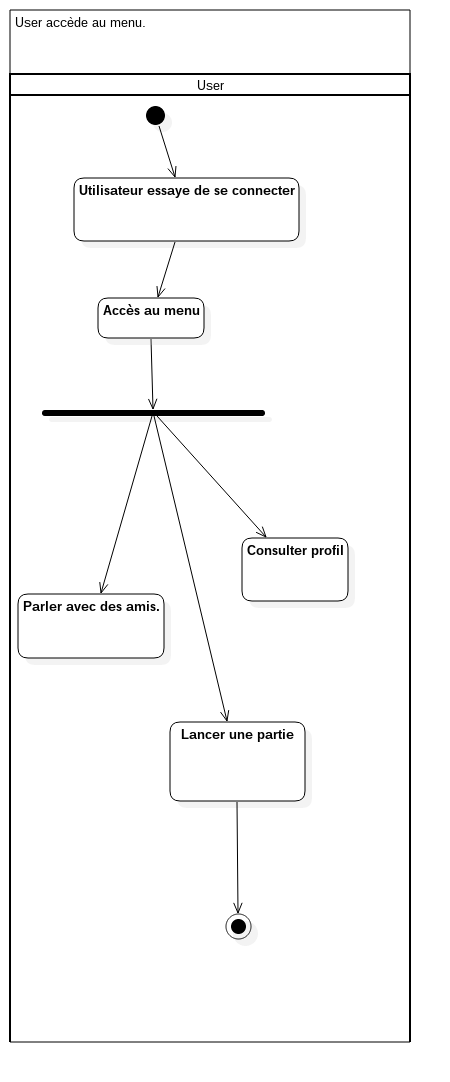
\includegraphics[height=17cm,width=10cm]{user_serveur_diagramme.png}
 
 \end{center}
   
\newpage
\subsection{Use case: en jeu}

\subsubsection{Use case diagramme en jeu:}

\begin{center}
    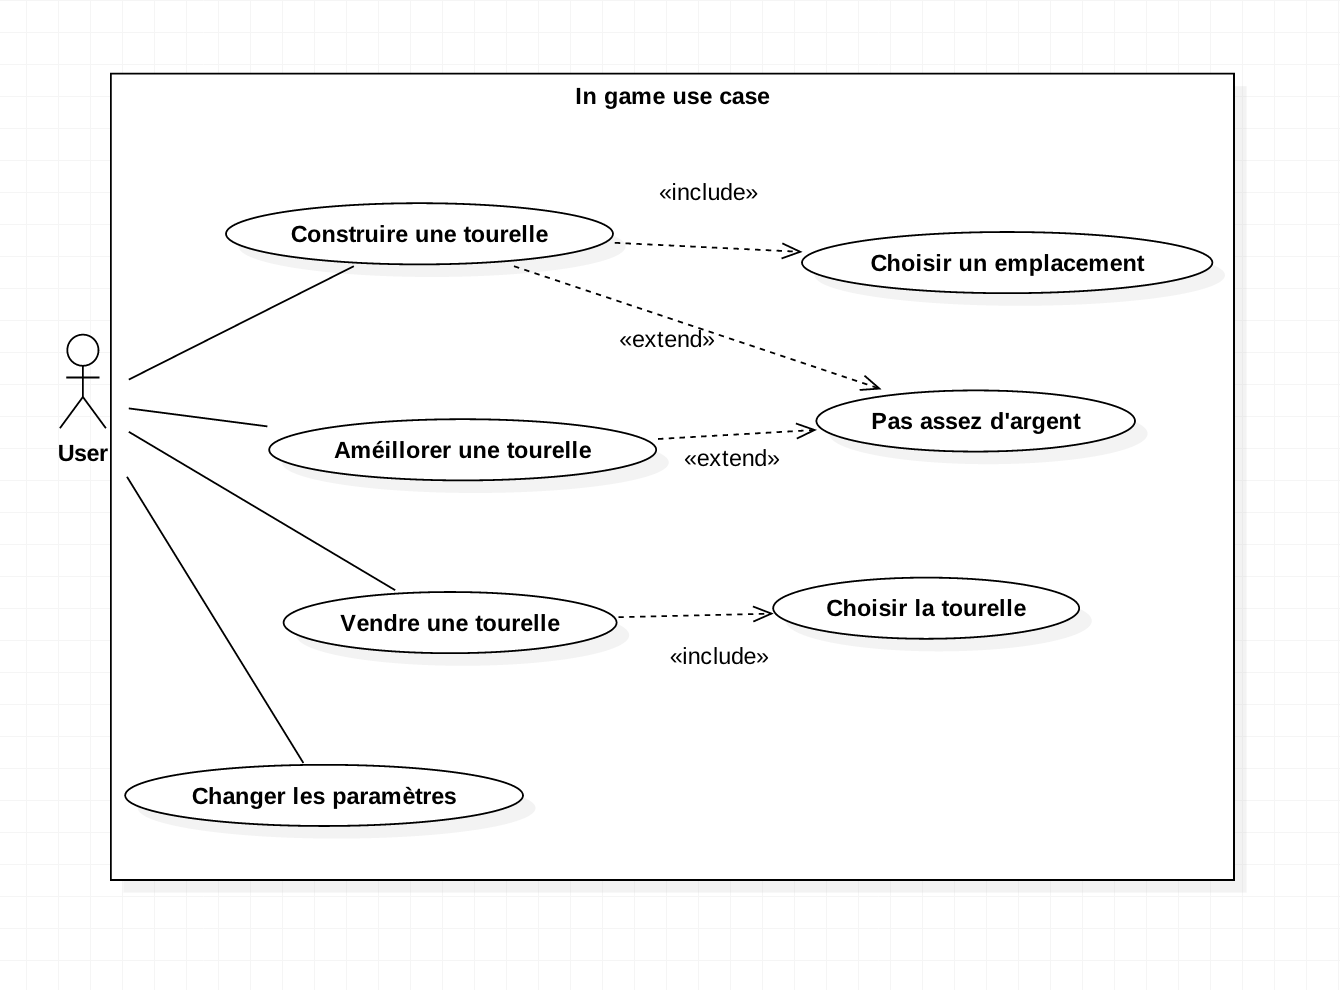
\includegraphics[height=13.5cm,width=17cm]{ingame_use_case.png}
\end{center}

%\newpage
\begin{itemize}
\item \textit{\textbf{Acteurs}} : ce deuxième use case a comme unique et principal acteur le \gls{joueur}.\\

\item \textit{\textbf{Préconditions}} : pour ce qui est des préconditions le \gls{joueur} doit être connecté et a dû lancer une partie\index{partie} via le \gls{serveur}.\\

\item \textit{\textbf{Postconditions}} : la seule postcondition est qu'une fois la partie\index{partie} terminée, le \gls{joueur} retourne au menu\index{menu}.\\

\item \textit{\textbf{Flux d'exécution}} : pour ce qui est du déroulement basique, une fois en jeu le \gls{joueur} peut construire des tourelles, consulter la description de celles-ci, il peut également les améliorer, les vendre, mais aussi modifier les paramètres du jeu. Il existe également un flux d'exécution alternatif. Au lieu de jouer, l'\gls{utilisateur} peut être tout simplement un spectateur de la partie\index{partie}.

\end{itemize}


\newpage
\subsubsection{Diagramme d'activité lors que le joueur est en jeu:}

\begin{center}
    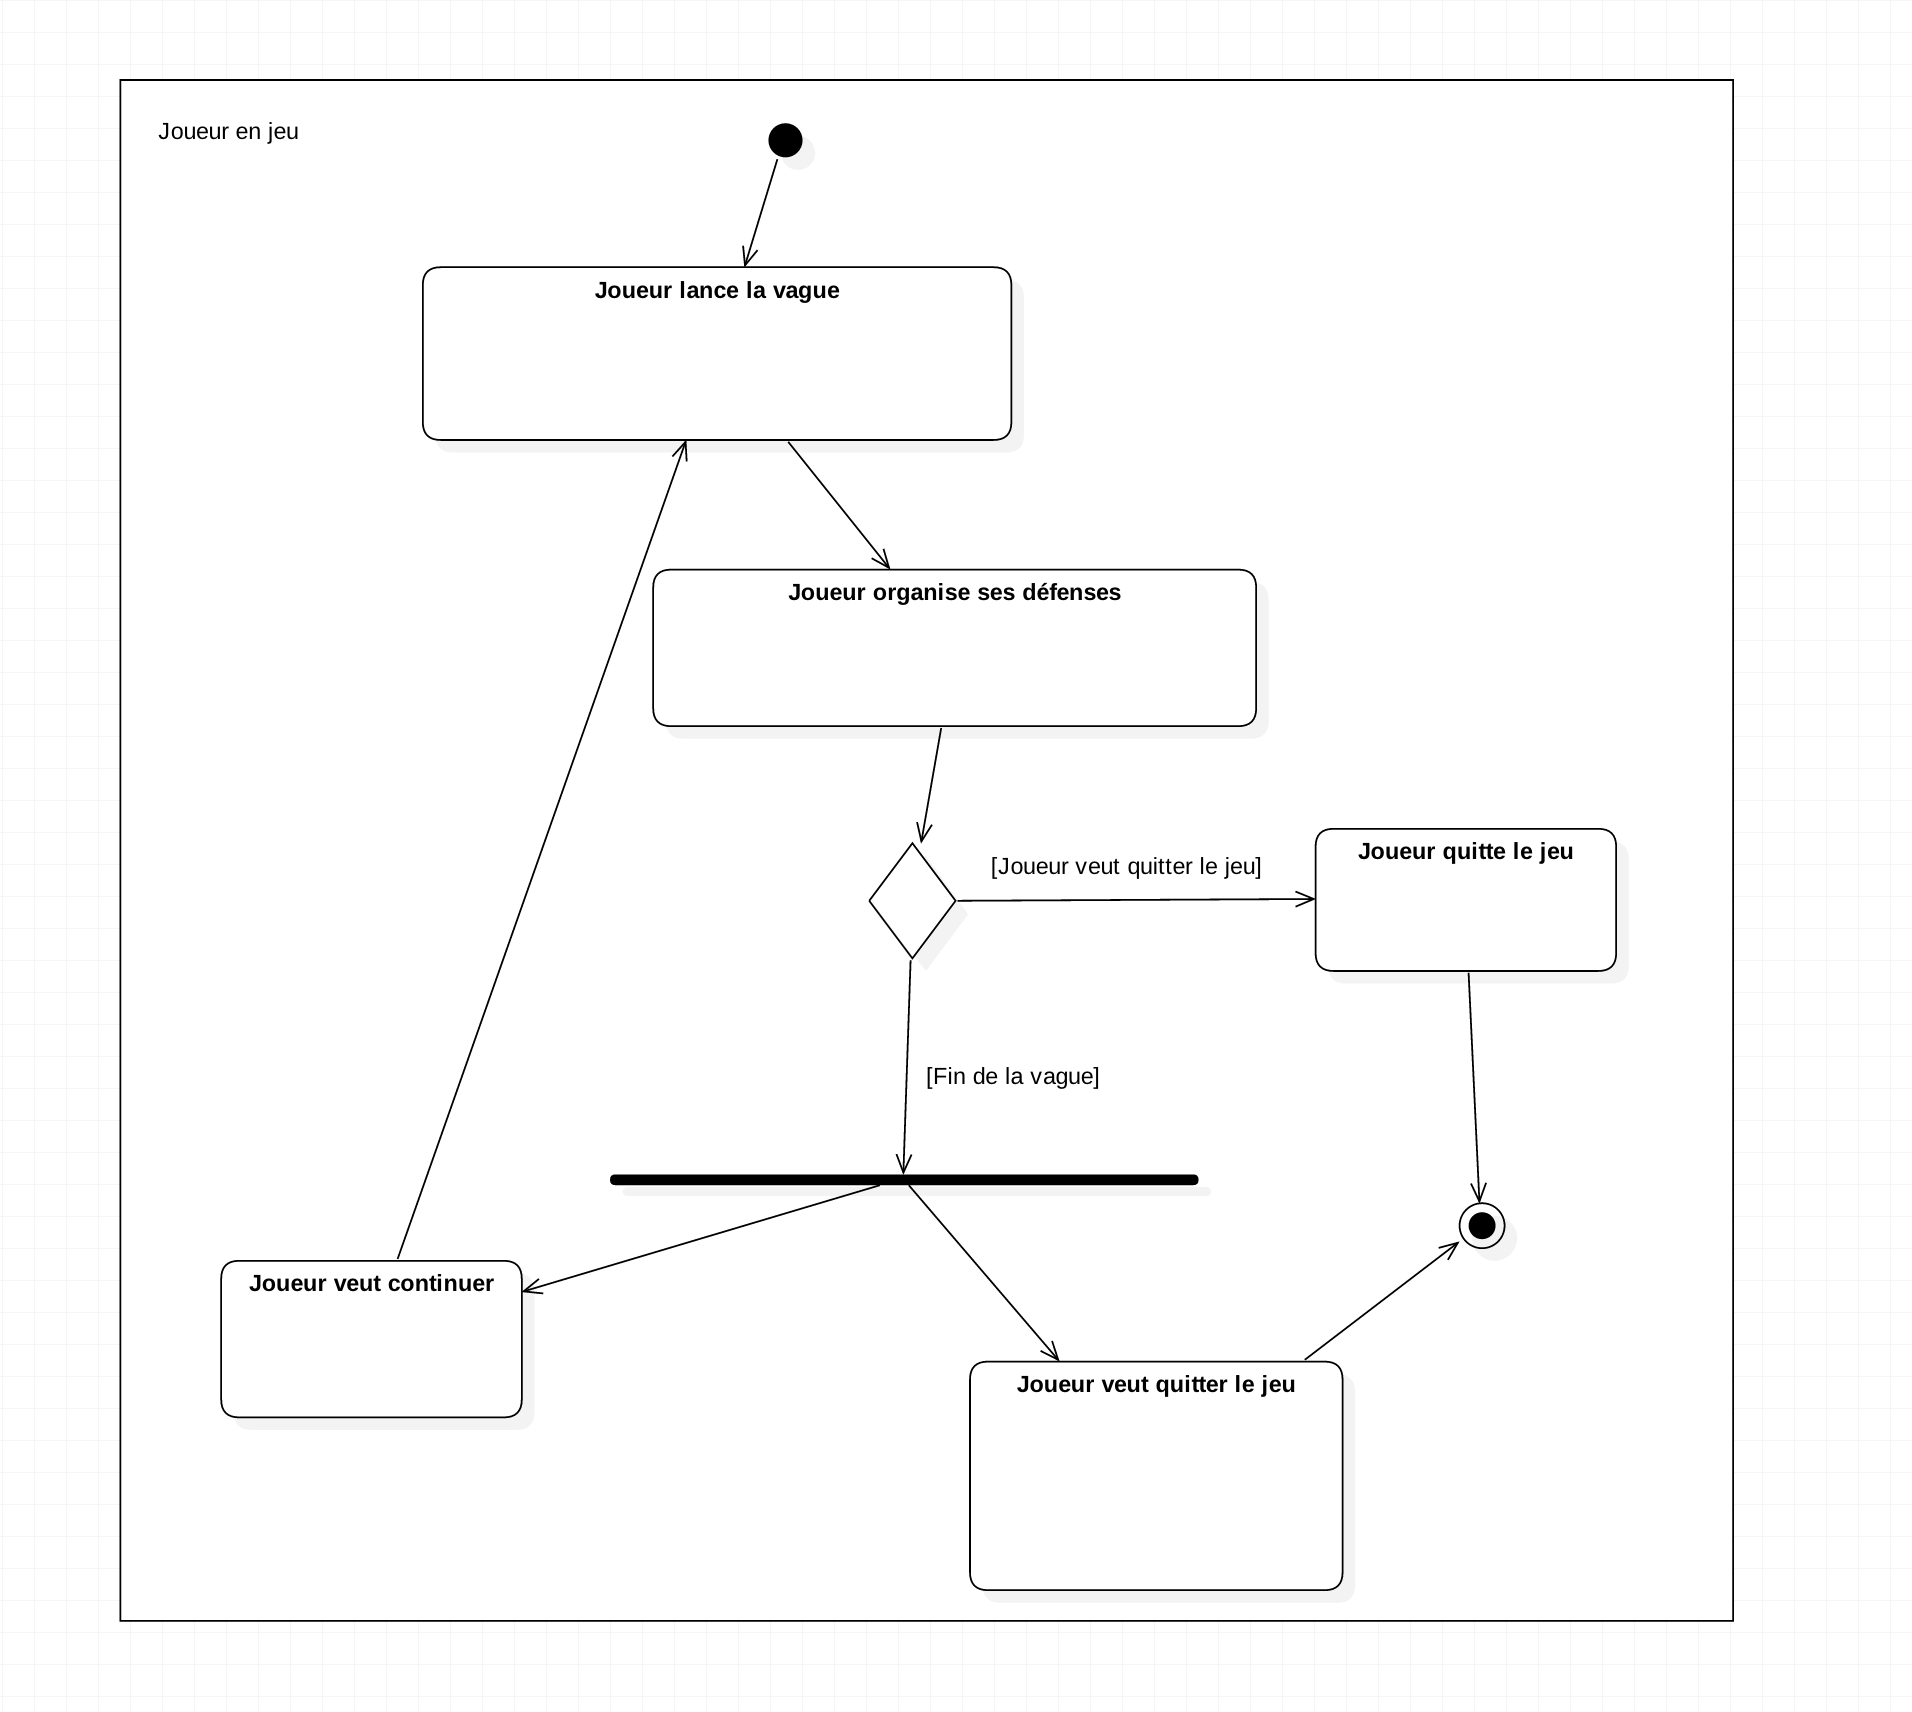
\includegraphics[height=16cm,width=19cm]{joueur_en_jeu.png}
\end{center}

\newpage    
\subsection{Exigences non fonctionnelles}

\begin{itemize}
    \item Menu\index{menu} et interface intuitifs.
    \item Animations graphiques.
    \item Animations sonores
    \item Maniabilité
    
\end{itemize}
    
\subsection{Exigence de domaine}

\begin{itemize}
	\item Le jeu doit être multijoueur, les différents \glspl{utilisateur} connectés sur un même \gls{serveur} doivent pouvoir agir sur le terrain.
   \item  L'abandon\index{abandon} d'un des \glspl{joueur} ne doit pas empêcher les autres de terminer leur partie\index{partie}. 
   \item Un jeu de Tower Defense est un jeu de 2 à 4 \glspl{joueur} qui ont chacun une partie\index{partie} de la carte.
   \item Chacun des \glspl{joueur} a sa base\index{base} dans chaque coin du jeu.
   \item Les ennemis\index{ennemis} apparaissent au milieu de la carte, leur vagues sont identiques pour chaque \gls{joueur}.
   \item La partie\index{partie} se déroule sous forme de vagues successives d’ennemis\index{ennemis} jusqu’à ce que la partie\index{partie} se termine.
   \item  Les \glspl{joueur} peuvent améliorer ou acheter des tours à tout moment de la partie\index{partie}.
   \item  La partie se termine si le temps est écoulé dans le cas d’une partie\index{partie} en mode chrono\index{mode chrono} ou s’il ne reste qu’un \gls{joueur} vivant dans le cas d’une partie classique\index{partie classique}.
\end{itemize}
\newpage
\section{Besoin du système}
\subsection{Exigences fonctionnelles}
\subsubsection{Use case diagramme des exigences fonctionnelles :}

\begin{center}
    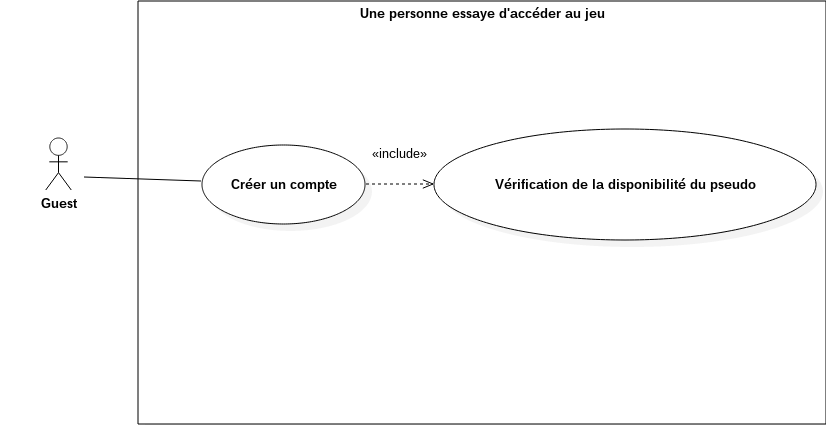
\includegraphics[height=10cm,width=15cm]{personne_acces_jeu.png}
\end{center}

\subsubsection{Use case: Connexion au jeu}

\begin{description}
	\item[cas général :] L'\gls{utilisateur} doit pouvoir se connecter en utilisant son nom d'\gls{utilisateur} et son mot de passe.
    \item[Pré condition :] L'\gls{utilisateur} n'est pas encore connecté.
    \item[Post condition :] L'\gls{utilisateur} s'est connecté.
    \item[Cas exceptionnel :] L'authentification échouera et l'\gls{utilisateur} sera invité a recommencer si son mot de passe ou son num d'\gls{utilisateur} est mauvais.
\end{description}
\newpage
%\par Ce use case à comme acteur principal un utilisateur, mais aussi un acteur secondaire qui est le guest.\\

%\par Pour ce qui est des préconditions il y en a qu'une seule pour un utilisateur, à savoir que celui-ci ai un compte valide. La seule postcondition est que l'utilisateur ou le guest soit connecté.\\
%\par Ensuite, pour ce qui est du déroulement basique, l'utilisateur va essayer de se connecter et le système le fait accéder au jeu. Pour ce qui est du guest, celui-ci fait une demande au système pour créer un compte, le serveur crée le compte et fait accèder le nouvel utilisateur au jeu.\\
	
%\par 
%	Pour ce qui est du déroulement alternatif, du côté de l'utilisateur, si celui-ci entre un compte invalide ou un mot de passe incorrect, il se verra refuser l'accès au jeu par le serveur. Du côté du guest, si le pseudo est déjà pris, il recevra une nouvelle demande de création de compte.\\

\subsubsection{Use case : lancer une partie\index{partie}}
\subsubsection{Use case diagramme de lancer une partie:}	
\begin{center}
    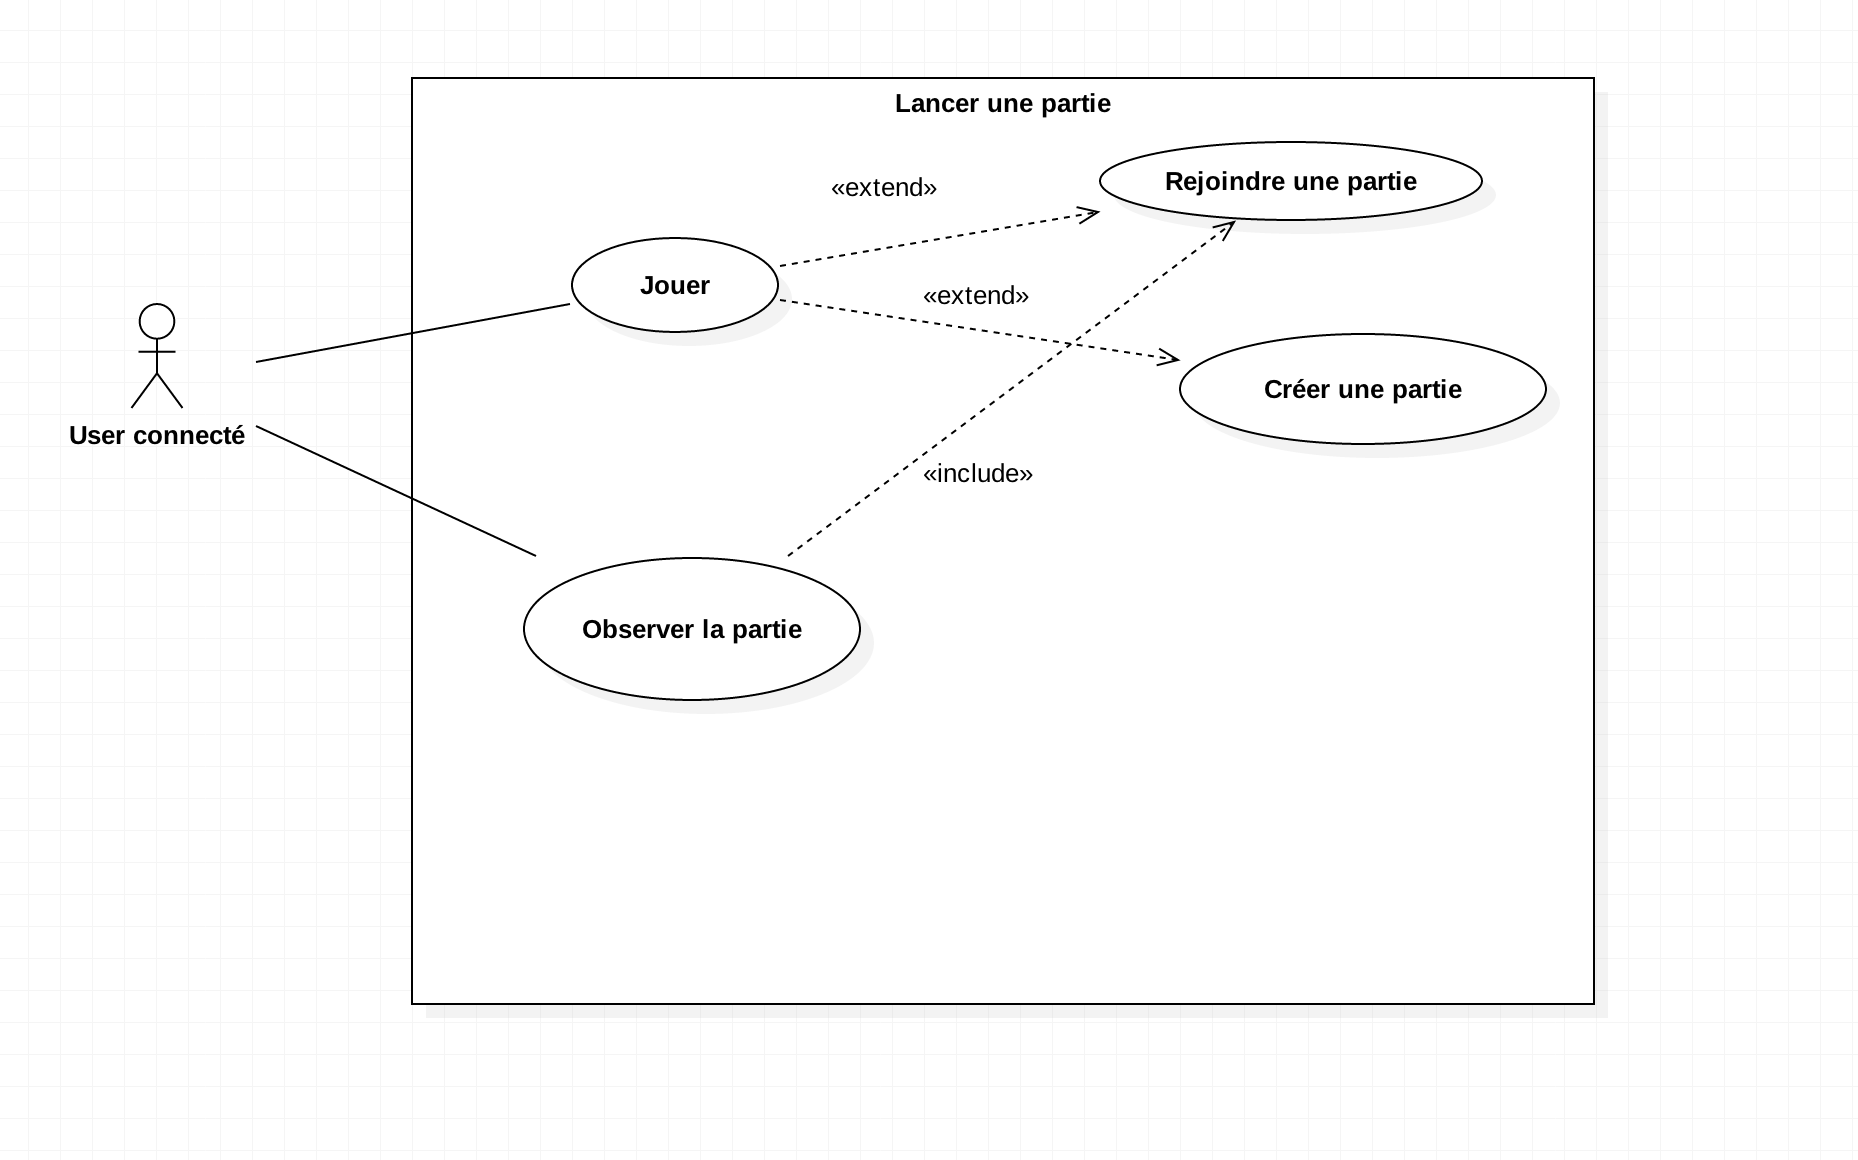
\includegraphics[height=13cm,width=19cm]{lancer_une_partie.png}\index{partie}
\end{center}
\begin{itemize}
\item \textit{\textbf{Acteurs}} : pour ce use case, le seul acteur est l'utilisateur ayant un compte.\\

\item \textit{\textbf{Préconditions}} : en ce qui concerne les préconditions, il y en a qu'une seule à savoir que le système ai bien trouvé le compte de l'utilisateur et l'ai fait accéder au jeu.\\

\item \textit{\textbf{Postconditions}} : pour ce qui est des postconditions, l'utilisateur doit avoir rejoins un salon de jeu ou avoir créé un salon ou encore rejoins une partie\index{partie} en tant que spectateur.\\

\item \textit{\textbf{Flux d'exécution}} : pour ce qui est du flux d'exécution basique, Le joueur va soit rejoindre une partie\index{partie} grâce au système qui lui trouve un salon libre, soit créer une partie\index{partie}. Il peut finalement rejoindre une partie\index{partie} en tant que spectateur grâce au système qui lui trouve une partie\index{partie} déjà lancée. \\

\end{itemize} 
\newpage

\subsubsection{Use case diagramme:}	
\begin{center}
    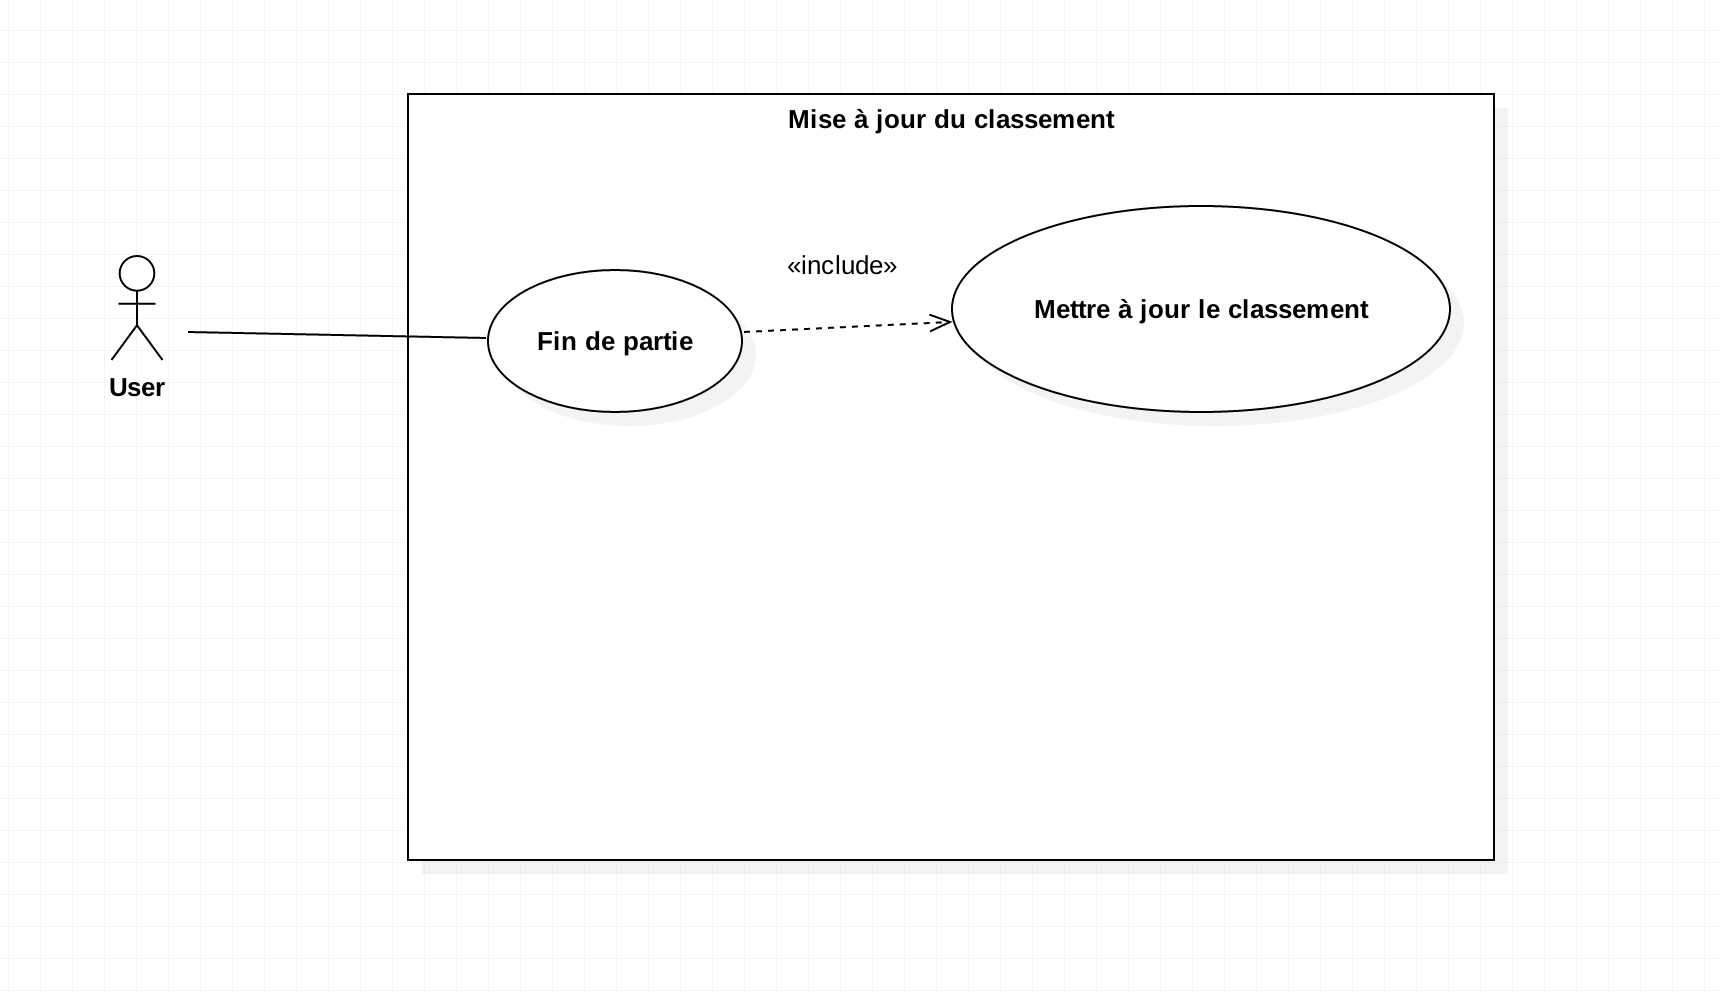
\includegraphics[height=14cm,width=17cm]{maj_classement.png}
\end{center}
\begin{itemize}

\item \textit{\textbf{Acteurs}} : pour ce use case, il n'y a pas vraiment d'acteurs qui entrent en jeu. Le système se chargera de tout.\\

\item \textit{\textbf{Préconditions}} :pour ce qui est des précondtions, la seule et unique précondition est que l'utilisateur était dans une partie\index{partie} en tant que joueur et non en tant que support.\\

\item \textit{\textbf{Postconditions}} : pour les postcondtions, il faut que la partie\index{partie} se soit bien totalement terminée.\\

\item \textit{\textbf{Flux d'exécution}} : en ce qui concerne du flux d'exécution basique, Le joueur va jouer sa partie\index{partie} la partie\index{partie} se termine et le système va mettre à jour le classement\index{classement} si besoin.\\
\end{itemize}

\newpage

\subsubsection{Use case : User dans le salon de discussion}
\subsubsection{Use case diagramme:}	

  
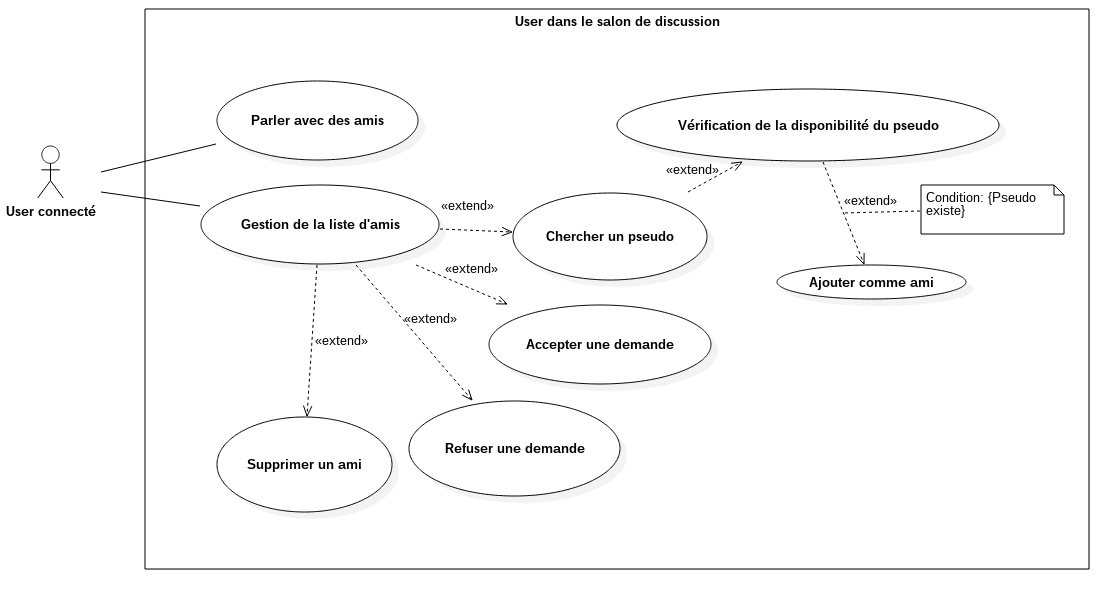
\includegraphics[height=13cm,width=18.5cm, left]{user_salon_de_discussion.png}
	
%\newpage

\par Ce dernier use case ne comporte qu'un seul acteur, il s'agit de l'utilisateur.\\

\par Pour ce qui est des préconditions, l'utilisateur a dû être capable de se connecter et d'avoir lancé le salon de discussion. Ensuite, pour ce qui est des postconditions, aucune n'entre en jeu.\\

\par Le flux d'exécution basique dans ce dernier use se déroule de la manière suivante :
Le joueur/utilisateur va soit vouloir parler avec un ami, au quel cas le système va ouvrir un salon de discussion entre le joueur et son ami. Par ailleur, il peut également vouloir organiser sa liste d'amis\index{liste d'amis}, ce qui mène à plusieurs cas dont le système se chargera. Ces cas sont :
\begin{itemize}
	\item Le joueur recoit une demande d'amis et l'accepte ou la refuse.
    \item Le joueur envoie une demande d'amis.
    \item Le joueur supprime un ami.
\end{itemize}
\newpage	

\subsection{Exigences non fonctionnelles}

\begin{itemize}
    \item Portabilité. 
    \item Optimisation du code 
    \item Organisation 
    \item Réactivité 
\end{itemize}
%\newpage
\subsection{Design et fonctionnement du système}
  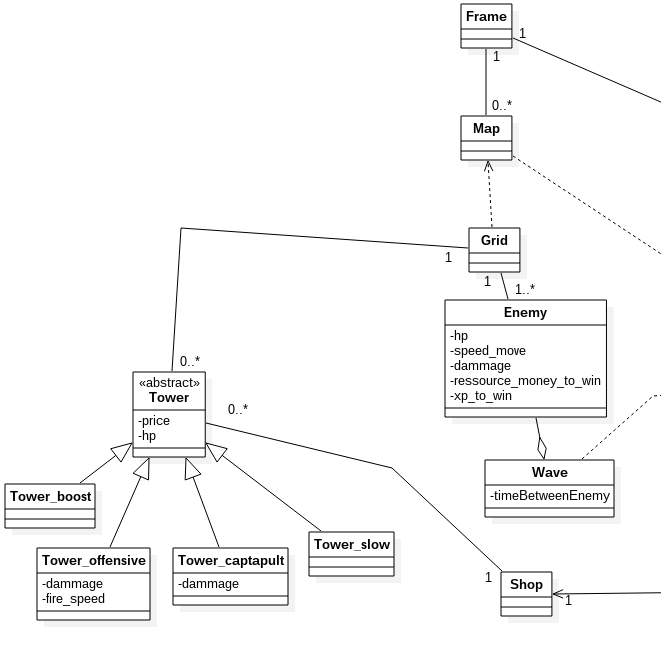
\includegraphics[height=16cm,width=16cm]{Class_ingame.png} 
  \newpage
	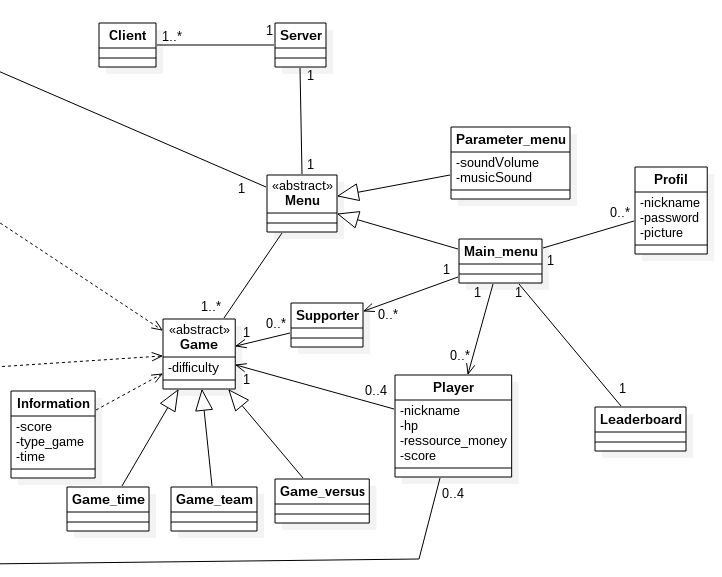
\includegraphics[height=16cm,width=16cm]{Class_menu.png}\index{menu}
\newpage
\subsubsection{Diagramme de sequence d'une connection}
  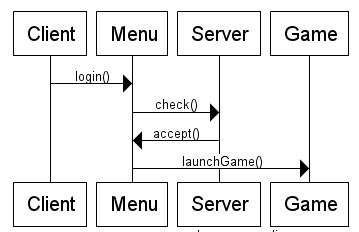
\includegraphics[height=9.5cm,width=16cm]{sequence.png} 

\newpage


%\section{Index et termes utilisés}
\printindex

\end{document}